\documentclass[10pt]{beamer}
%\documentclass[10pt, handout]{beamer}
\setbeameroption{show notes}

%\documentclass[10pt, a4paper]{article}
%\usepackage{beamerarticle}




\mode<article>{
	
	\usepackage{hyperref}
	
}
\mode<presentation>{
	
	\usetheme{Antibes}
	\usefonttheme{professionalfonts} 
	\usefonttheme{serif} % default family is serif
	
	%\usecolortheme{spruce} %зеленая, плохой цвет в заголовках 
	%\usecolortheme{albatross} %синяя, пхоло виден черный цвет
	
}

\newcommand{\MP}[1]{\mode<presentation>{#1} }
\newcommand{\MA}[1]{\mode<article>{#1} }

\newcommand{\ABS}[1]{\left| #1 \right|}
%\newcommand{\ABS}[1]{\mid #1 \mid}

\newcommand{\HREF}[2]{{\color{blue}\underline{\href{#1}{#2}}}}

\setbeamertemplate{caption}[numbered]


%\usepackage[T2A]{fontenc}
%\usepackage[utf8]{inputenc}
%\usepackage[russian]{babel}
%\usepackage{amsmath} %математические формулы



\usepackage{ifthen}

\usepackage{tikz}
\usetikzlibrary{arrows.meta}
\usetikzlibrary{calc}
\usetikzlibrary{decorations}
\usetikzlibrary{decorations.pathreplacing}
\newcommand{\rememb}[1]{\tikz[remember picture,baseline=-0.5ex]{\draw node[inner sep=0pt, outer sep=0pt] (#1){\strut};}}



\usepackage{fp}
\usepackage{tikz-3dplot}
\usepackage{environ}
\usepackage{animate}





\usepackage{xcolor}
%\usepackage[left=20mm,right=20mm,top=20mm,bottom=20mm,a4paper]{geometry} %поля

\usepackage{amsmath} %математические формулы
%\usepackage{amsfonts} %математические шрифты


\usepackage[e]{esvect}  %Красивая стрелочка вектора
%\let\oldvv\vv
\newcommand{\VV}[1]{\vv{#1\mathstrut}}



\usepackage{graphicx} %работа с каритнками


%\usepackage{multimedia}
%\usepackage{movie15}

%Для XeLatex/+
\usepackage{polyglossia}
\setdefaultlanguage{russian}
\setotherlanguage{english}
%\setkeys{russian}{babelshorthands=true} 


\usepackage{fontspec}

\setmainfont{Times New Roman} [Script=Cyrillic, Mapping=tex-text,]
\setsansfont{Arial} [Script=Cyrillic, Mapping=tex-text,]
%\setmonofont{Courier New} [Script=Cyrillic, Mapping=tex-text,]
\newfontfamily{\cyrillicfonttt}{Courier New}


%\usepackage{unicode-math}
%\setmathfont{TeX Gyre Termes Math}

%\setmainfont{CMU Serif}[Script=Cyrillic, Mapping=tex-text,]
%\setsansfont{CMU Sans Serif}[Script=Cyrillic, Mapping=tex-text,]
%\setmonofont{CMU Typewriter Text}[Script=Cyrillic, Mapping=tex-text,]


%-----------------


%\usepackage{caption}
%\DeclareCaptionLabelSeparator{dot}{~---~}            %Разделитель номер рисунка
%\captionsetup[figure]{justification=centering,labelsep=dot, format=plain}                        %Подпись рис. центр
%\captionsetup[table]{justification=raggedleft,labelsep=dot, format=plain, singlelinecheck=false} %Подпись табл. слева
%\captionsetup[lstlisting]{justification=raggedleft,labelsep=dot, format=plain, singlelinecheck=false}                     %Подпись рис. центр

\usepackage{indentfirst} %отступ первой строки


\usepackage[svgnames]{xcolor}


\usepackage{hyperref}

%\usepackage{showframe}


%\usepackage{tikz}

%\usepackage[hidelinks]{hyperref}%ссылки внутри документа \ref


\setlength\abovecaptionskip{-2pt}
%\setlength\belowcaptionskip{-14pt}

\setbeamerfont{caption}{size=\scriptsize}


\def\sectionname{Раздел}
\def\subsectionname{Подраздел}


\newcommand{\TC}[3]
{
	
	
	\begin{columns}
		\begin{column}{#1\textwidth}
			#2
		\end{column}
		\begin{column}{\fpeval{1-#1}\textwidth}
			#3
		\end{column}
	\end{columns}
}

\newcommand{\TCT}[3]
{
	
	\begin{columns}[T]
		\begin{column}{#1\textwidth}
			#2
		\end{column}
		\begin{column}{\fpeval{1-#1}\textwidth}
			#3
		\end{column}
	\end{columns}
}


\newcommand{\FRAME}[2]{
	\begin{frame}
		\frametitle{#1}
		#2
	\end{frame}
}

\newcommand{\FIG}[3]
{
	\begin{figure}
		\centering
		\includegraphics[width=#3]{#1}
		\caption{#2}
	\end{figure}
}

\newcommand{\vect}[1]{\overrightarrow{#1}}


\usepackage{qrcode}

\newcommand{\LECADDR}{https://clck.ru/3D3Efj}


\usepackage{newfile}

\edef\LectionNumber{0}
\edef\LectionTheme{0}

\let\oldsection\section
\let\oldsubsection\subsection


\AtBeginDocument
{
	\newoutputstream{CONTENT}
	\openoutputfile{\LectionNumber .gvr}{CONTENT}
	
	\expandafter\addtostream{CONTENT}{\noindent\textbf{\Large Лекция \LectionNumber~---~\LectionTheme}\unexpanded{\setcounter{SEC}{0}}\par}
}

\renewcommand{\section}[1]{
	\oldsection{#1}
	\expandafter\addtostream{CONTENT}{\noindent\hspace{2ex}\unexpanded{\hbox{\large\stepcounter{SEC}\theSEC ~ #1}}\par}
}

\renewcommand{\subsection}[1]{
	\oldsubsection{#1}
	\expandafter\addtostream{CONTENT}{\noindent\hspace{6ex}\unexpanded{\stepcounter{SUB}\theSUB ~ #1}\par}
}


%\renewcommand{\section}[1]{\MMM{#1}}

%\edef\subsection#1
{
	%\noexpand\subsection{#1}
	%
}


\newfontfamily\dnifamily[Scale = 0.795]{DniFont.TTF}

\newcommand{\dni}[1]{%
	{\dnifamily%
		\ifthenelse{#1=0}{0}{}%
		\ifthenelse{#1=1}{1}{}%
		\ifthenelse{#1=2}{2}{}%
		\ifthenelse{#1=3}{3}{}%
		\ifthenelse{#1=4}{4}{}%
		\ifthenelse{#1=5}{5}{}%
		\ifthenelse{#1=6}{6}{}%
		\ifthenelse{#1=7}{7}{}%
		\ifthenelse{#1=8}{8}{}%
		\ifthenelse{#1=9}{9}{}%
		\ifthenelse{#1=10}{)}{}%
		\ifthenelse{#1=11}{!}{}%
		\ifthenelse{#1=12}{@}{}%
		\ifthenelse{#1=13}{\#}{}%
		\ifthenelse{#1=14}{\$}{}%
		\ifthenelse{#1=15}{\%}{}%
		\ifthenelse{#1=16}{\^{}}{}%
		\ifthenelse{#1=17}{\&}{}%
		\ifthenelse{#1=18}{*}{}%
		\ifthenelse{#1=19}{(}{}%
		\ifthenelse{#1=20}{[}{}%
		\ifthenelse{#1=21}{]}{}%
		\ifthenelse{#1=22}{\textbackslash{}}{}%
		\ifthenelse{#1=23}{\{}{}%
		\ifthenelse{#1=24}{\}}{}%
		\ifthenelse{#1=25}{|}{}}%
}%

\newcommand{\toDni}[1]{%	
	\ifthenelse{#1=0}{}{%
		 \ifthenelse{#1=25}{%
		 	\expandafter\dni{#1}}{%
		 	\expandafter\toDni{\fpeval{floor(#1/25)}}%
		 \expandafter\dni{\fpeval{(#1/25 - floor(#1/25))/0.04}}}}%
}%



\newcommand{\Strut}{{\Large\strut}}

\newcommand\scb[1]{\left( #1 \right)}

\newcommand{\LINK}[2]{%
	\qrcode[height=1cm]{#1}\  \HREF{#1}{\parbox{0.8\textwidth}{#2}} \\[0.5em]
}

\NewDocumentCommand{\lecdni}{}{\toDni{\LectionNumber}}
\author{Гаврилов Андрей Геннадьевич}
\newcommand{\regals}{кандидат технических наук, доцент}
\institute{Кафедра Информационных технологий и вычислительных систем \\МГТУ~<<СТАНКИН>>}
\lecture{История компьютерной графики}{kghistory}\subtitle{Компьютерная графика}


\makeatletter
\newcommand*{\overlaynumber}{\number\beamer@slideinframe}
\makeatother



\usepackage{cprotect}

\newcommand{\QRFRAME}{%
    \begin{frame}[plain, noframenumbering]    	
	
	\centering
	Трансляция презентации (во время очных лекций)    
	
	~
	
	{\Large \ttfamily  https://clck.ru/3D3Efj  }
	
	~
	
	\tikz\node[inner sep=0pt,rounded corners=5mm, clip]{\qrcode[height=0.45\textwidth]{\LECADDR}}; 
	
	~	
	{\small
	При просмотре презентации в PDF для отображения анимаций на слайдах необходимо использовать Acrobat Reader, KDE Okular, PDF-XChange, Foxit Reader, браузер Firefox. Для браузеров на движке Chrome (Edge, Яндекс, Opera,~\dots) необходимо использовать \HREF{https://chromewebstore.google.com/detail/pdf-viewer/oemmndcbldboiebfnladdacbdfmadadm?hl=ru&utm_source=ext_sidebar}{PDF.js} c опцией <<Enable active content (JavaScript) in PDFs>>. }
	
	\end{frame}%
}

\newcommand{\IG}[2][1]{\includegraphics[width=#1\textwidth]{#2}}



\graphicspath{{Images/}{Images/\jobname/}}

\date{\today}



\renewcommand{\LectionNumber}{8}
\renewcommand{\LectionTheme}{Отсечение невыдимых граней}
\title{Лекция \lecdni \\ \LectionTheme}
\subtitle{Компьютерная графика}



%\usepackage{standalone}

\setbeamersize
{
	text margin left=0.5cm,
	text margin right=0.5cm
}

\usepackage{comment}


%	\transduration{2}
%   \transfade

 \begin{document}
 		 
	\makeatletter
\defbeamertemplate*{title page}{my theme}
{
	
	\hfill
	
	\begin{beamercolorbox}[wd=.9\paperwidth,center,]{title}%
		
	\end{beamercolorbox}%	
	
	\vbox to 1em {}
	
	\begin{beamercolorbox}[wd=.9\paperwidth,center,]{title}%
		\usebeamerfont{subtitle}%
		\hfill
		
		\insertsubtitle
		
		\usebeamerfont{title}%
		\inserttitle{} \\[0.5em]
		
		
		
	\end{beamercolorbox}%	
	\hfill\hfill
	
	\begin{beamercolorbox}[wd=.9\paperwidth,center,]{}%
		\usebeamerfont{author}%
		\hfill \\[0.5em]
		\insertauthor{} \\[0.5em]
		\regals
		    
		\vbox to 1em{}
		\usebeamerfont{institute}%
		\insertinstitute {}
		
		\vbox to 1em{}			
		{\; }\insertshortdate{}
		
	\end{beamercolorbox}%	
	\hfill\hfill
	
	\vbox to 5em{}
	
	
}
\defbeamertemplate*{footline}{my theme}{
	\leavevmode%
	\hbox{%
		\begin{beamercolorbox}[wd=.25\paperwidth,ht=3.25ex,dp=0ex,center,sep=1pt]{author in head/foot}%
			\usebeamerfont{author in head/foot}%
			\insertauthor 
			\beamer@ifempty{\insertshortinstitute}{}
		\end{beamercolorbox}%
		\begin{beamercolorbox}[wd=.65\paperwidth,ht=3.25ex,dp=0ex,center,sep=1pt]{title in head/foot}%
			\usebeamerfont{title in head/foot}\insertshortinstitute
		\end{beamercolorbox}%
		\begin{beamercolorbox}[wd=.1\paperwidth,ht=3.25ex,dp=0ex,center, sep=0.5pt]{date in head/foot}%
			\usebeamerfont{date in head/foot}
			\footnotesize \expandafter\toDni{\insertframenumber} / \expandafter\toDni{\inserttotalframenumber}
	\end{beamercolorbox}}%
}



\makeatother






%float page top aligment
\makeatletter
\setlength{\@fptop}{0pt}
\setlength{\@fpbot}{0pt plus 1fil}
\makeatother

\newcommand \abs[1] {\left| #1 \right|}

\everymath{\displaystyle}

    
    \QRFRAME	
	

	\frame{\maketitle}

	
	\begin{frame}{План лекции}
		\tableofcontents
	\end{frame}
	

	
	\begin{frame}{Алгоритмы удаления невидимых граней и поверхностей}
		
		\begin{enumerate}
			\item Работающие в пространстве экрана
			\item Работающие в пространстве объектов
			\item Комбинированные варианты
			
		\end{enumerate}
		
	\end{frame}
	
	
	
	\section{Метод плавающего горизонта}
	
	\begin{frame}{Метод плавающего горизонта}
		\centering%
		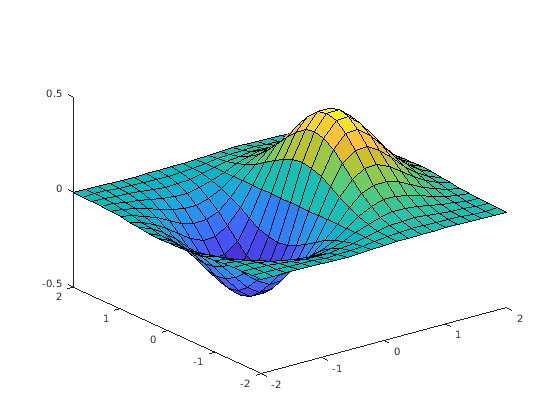
\includegraphics[width=0.8\textwidth]{CreateSurfacePlotExample_01.png}
	\end{frame}
	
	\begin{frame}{Метод плавающего горизонта}
		\TC{0.5}
		{
			\begin{enumerate}
				\item 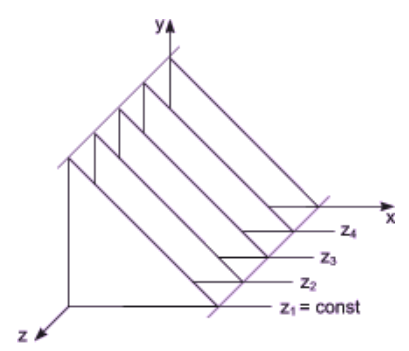
\includegraphics[width=0.8\textwidth]{mpg_1.png}
				\item 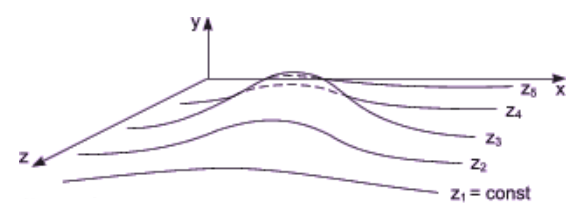
\includegraphics[width=0.9\textwidth]{mpg_2.png}
			\end{enumerate}
		}
		{
			\begin{enumerate}
				\setcounter{enumi}{2}
				\item 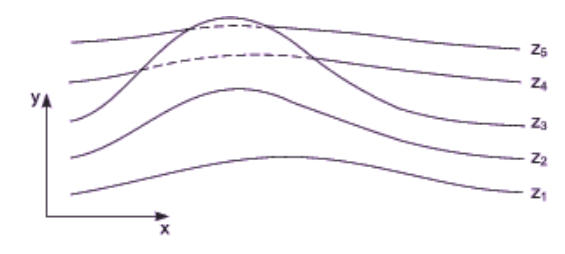
\includegraphics[width=0.9\textwidth]{mpg_3.png}
				\item 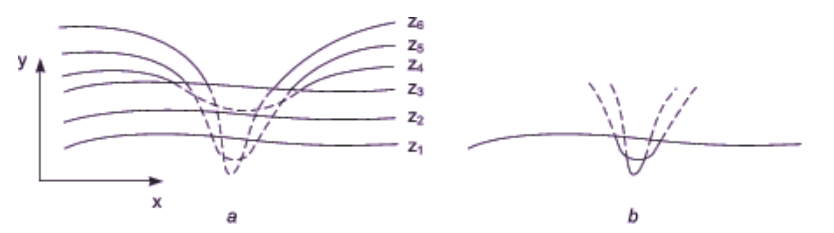
\includegraphics[width=0.9\textwidth]{mpg_4.png}
			\end{enumerate}
			
		}
		
	\end{frame}
	
	\begin{frame}{Примеры}
		
		\TC{0.5}
		{
			\centering%
			Пример хорошей отрисовки
			
			\fbox{\animategraphics[autoplay,loop, nomouse, width=0.85\textwidth]{5}{Images/\jobname/nikulin_good_draw/nikulin_good_draw-}{0}{69}}
		}
		{
			\centering%
			Пример плохой отрисовки
			\fbox{\animategraphics[autoplay,loop, nomouse, width=0.85\textwidth]{5}{Images/\jobname/nikulin_bad_draw/nikulin_bad_draw-}{0}{44}}
		}
		
		~
		
		\HREF{https://grafika.me/node/1093}{Демонстрация}
		
		
		
	\end{frame}
	

	
		
	\section{Отсечение нелицевых граней}
	
	
	\begin{frame}{Отсечение нелицевых граней}
		
	
			
			%\draw[very thin] (-5,-5) grid[step=0.5] (5,5);
%			\fill [red] circle (5pt);
%			\foreach \t in {-5,...,5}
%				{
%					\draw (\t,0) node {\t};
%					\draw (0,\t) node {\t};
%				}

			\TC{0.4}
			{
			\centering%
			\begin{tikzpicture}
						\coordinate (A) at (0,0);
			\coordinate (B) at (2,-1);
			\coordinate (C) at (3,0.2);
			\coordinate (D) at (0.9, 2);
			
			\draw (A) -- (B) -- (C) -- cycle;
			\draw (A) -- (D);
			\draw (B) -- (D);
			\draw (C) -- (D);
			
			\coordinate (G1) at (1,0.5);
			
			\draw [rotate=80, shift=(G1)]  circle[x radius = 0.3, y radius = 0.2];
			\draw[-Latex] (G1) -- +(170:1);
			
			\coordinate (G2) at (2,0.5);
			
			\draw [rotate=130, shift=(G2)]  circle[x radius = 0.3, y radius = 0.2];
			\draw[-Latex] (G2) -- +(20:1);
			
			\coordinate (G3) at (1.5,-0.3);
			
			\draw [rotate=0, shift=(G3),dashed]  circle[x radius = 0.3, y radius = 0.2];
			\draw[-Latex] (G3) -- +(-90:1);
			
			
			\coordinate (G4) at (1.2,1.1);
			
			\draw [rotate=0, shift=(G4),dashed]  circle[x radius = 0.25, y radius = 0.3];
			\draw[-Latex] (G4) -- +(120:0.7);
			
			\end{tikzpicture}
		}
		{
			
				\textbf{Для параллельной проекции}
				
					Для каждой грани $f$ необходимо проверить знак $\vv n \cdot \vv v$. 
					
					
					$\vv n \perp f$, $\vv v$ - вектор на наблюдателя ($\perp$ к плоскости проецирования)
				
				~
				
				
				\textbf{Для центральной проекции}
				
				Для каждой грани $f$ необходимо проверить знак $\VV n \cdot \VV{(c-p)}$. 
				
				$p \in f$, $c$ --- центр проекции.
	
		}
				

		
	\end{frame}
	
	\section{Алгоритм Робертса}
	
	\begin{frame}{Алгоритм Робертса}
		\centering%
		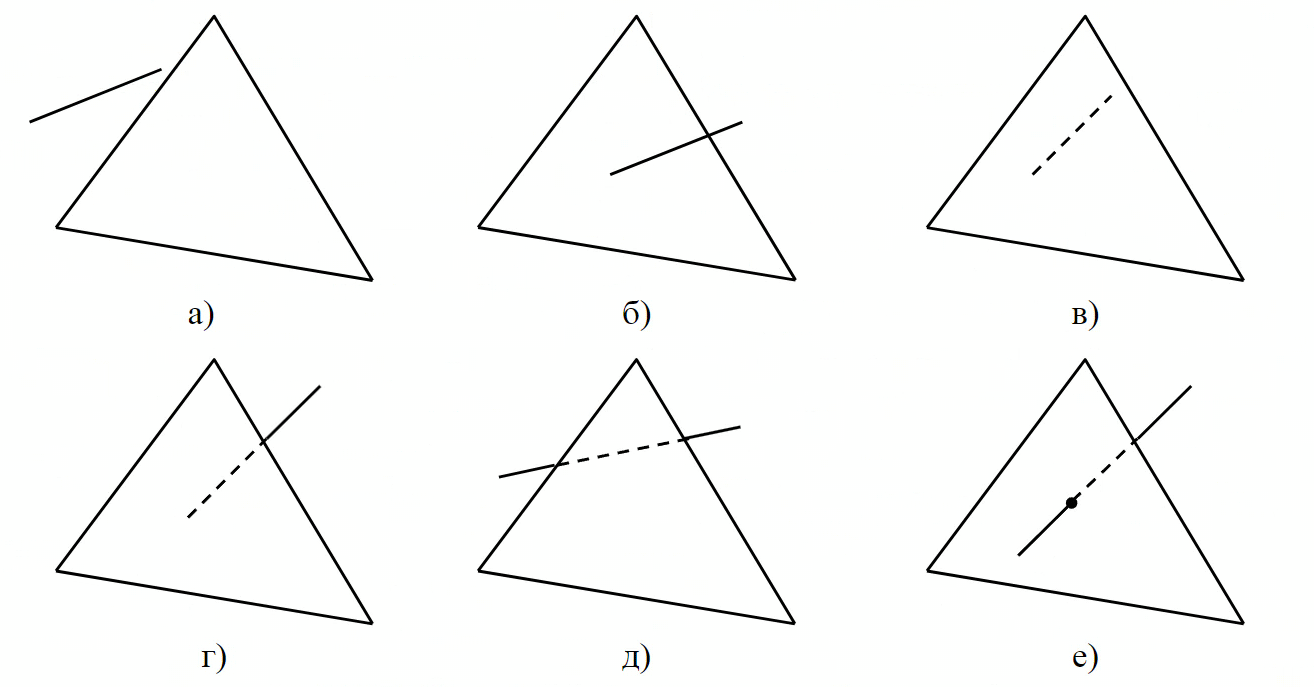
\includegraphics[width=0.9\textwidth]{roberts.png}
	\end{frame}
	
		\begin{frame}{Оптимизация алгоритма Робертса}
		\centering%
		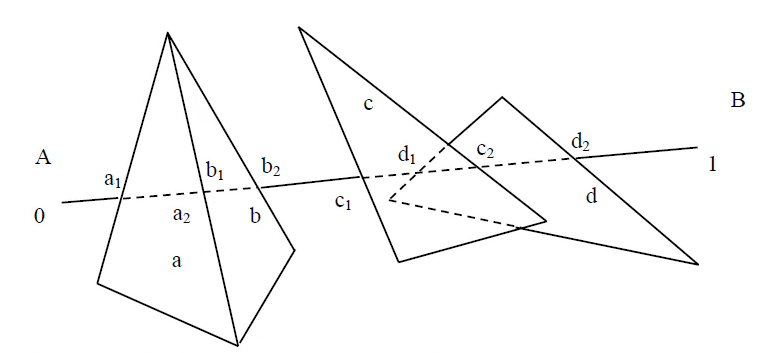
\includegraphics[width=0.9\textwidth]{roberts_opt2.png}
	\end{frame}
	
		\begin{frame}{Оптимизация алгоритма Робертса}
		\centering%
		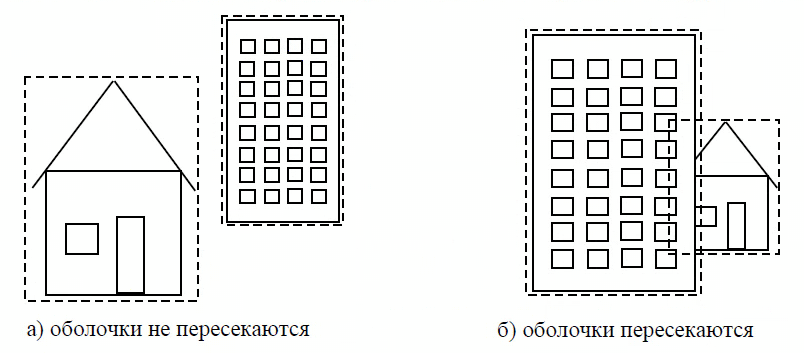
\includegraphics[width=0.9\textwidth]{roberts_opt.png}
	\end{frame}
	
	
	\section{Алгоритм Уорнока}
	
	\begin{frame}{Алгоритм Уорнока}
		\TC{0.45}
		{
			\centering%
			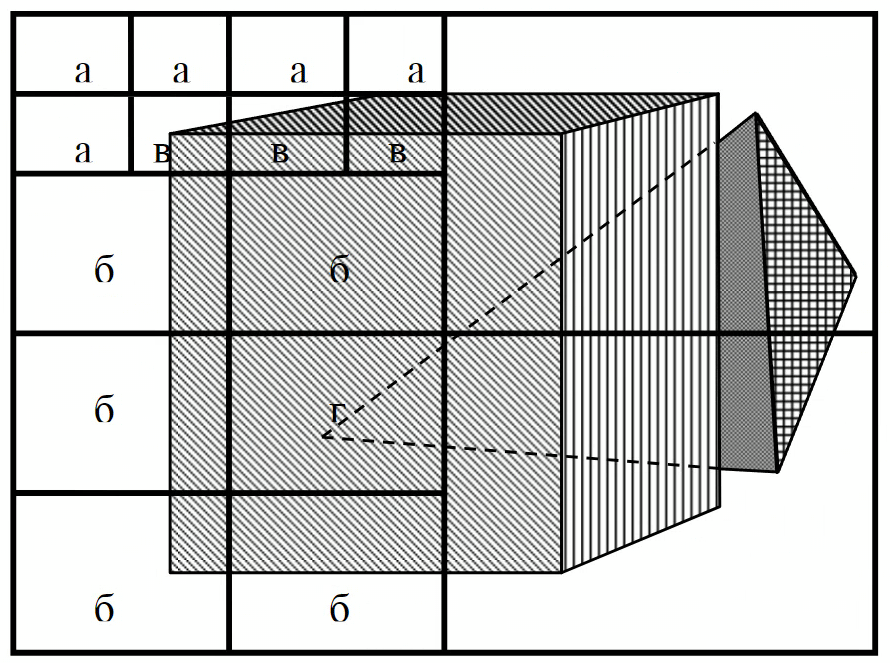
\includegraphics[width=1\textwidth]{varnak.png}	
		}
		{
			Случаи, когда можно легко определить видимость:
			\begin{itemize}				
			
			\item окне нет ни одной грани, в этом случае ничего рисовать не нужно;
			\item в окне ровно одна грань, в этом случае достаточно отобразить эту
			грань;
			\item размеры окна равны размерам одного пиксела, в этом случае из
			граней выбирается ближайшая;
			\item ближайшая грань охватывает всё окно, в этом случае она заслоняет все остальные грани.
			
			\end{itemize}
		}
		
		Алгоритм можно разделить на следующие элементарные задачи:\\
		- определение, в какие части окна попадает грань;\\
		- определение, что грань охватывает окно;\\
		- определение, что грань является ближайшей.
	\end{frame}
	
	\begin{frame}{Разделение окна вдоль общего ребра двух граней}
		\centering%
		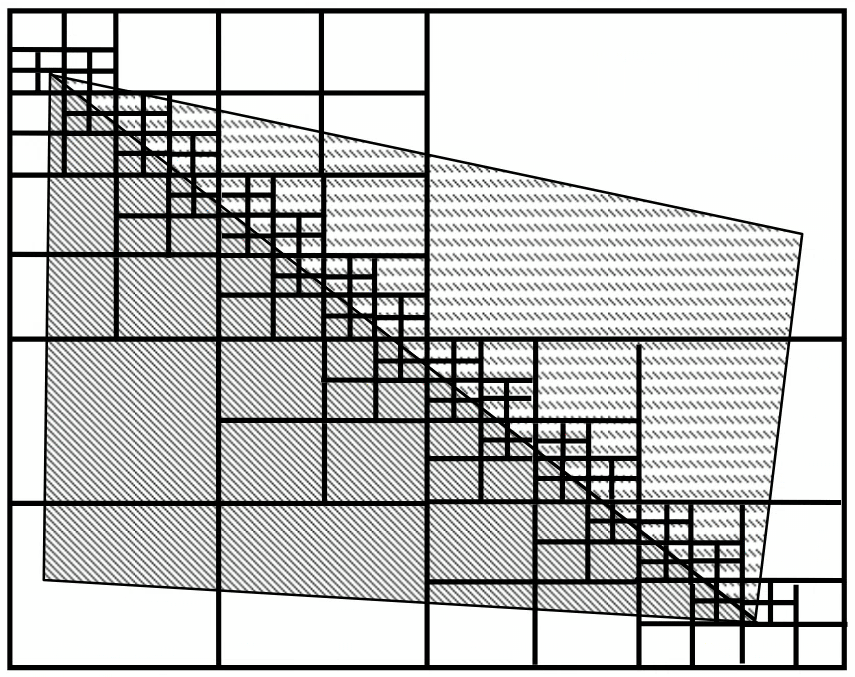
\includegraphics[width=0.7\textwidth]{varnak2.png}	
	\end{frame}
	
	\section{Алгоритм Z-буфера}
	
	\begin{frame}{Алгоритм Z-буфера}
		\TC{0.65}
		{
			\centering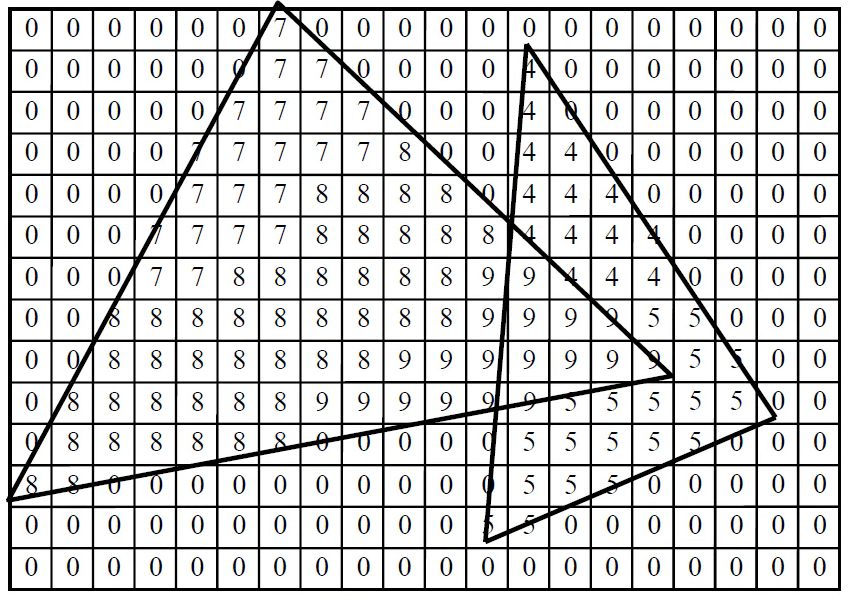
\includegraphics[width=0.95\textwidth]{zbuffermatrix.png}
		}
		{
			\centering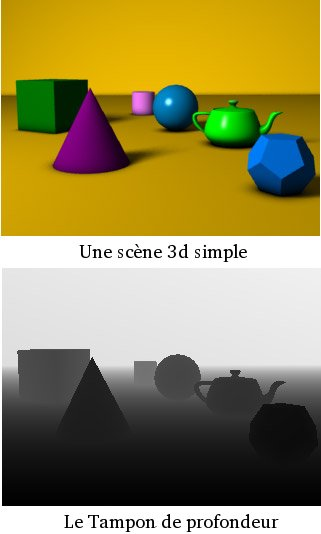
\includegraphics[width=0.95\textwidth]{Z-buffer_example.jpg}
		}
	\end{frame}
	
	\section{Алгоритм художника}
	
	\begin{frame}{Алгоритм художника}
		\TC{0.7}		
		{\centering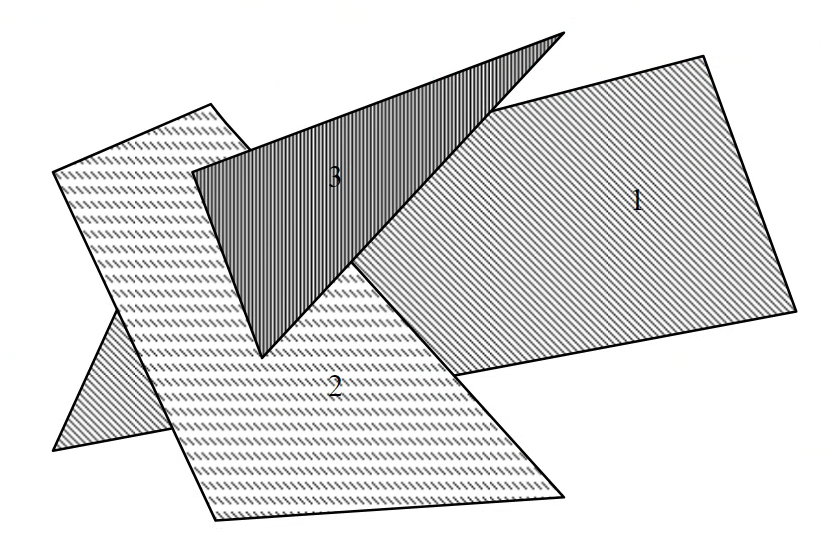
\includegraphics[width=\textwidth]{artist.png}}		
		{\centering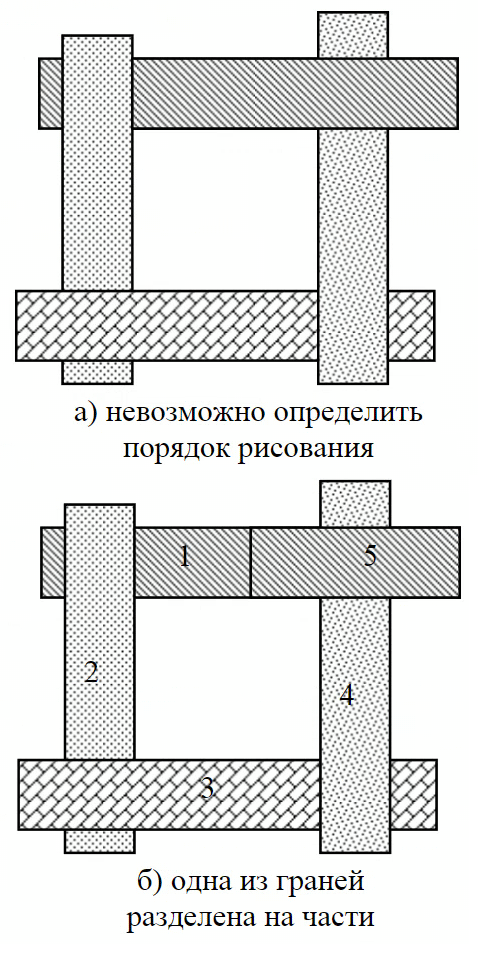
\includegraphics[width=\textwidth]{artist2.png}}
		
	\end{frame}
	
	
		\begin{frame}{Алгоритм художника}
	\centering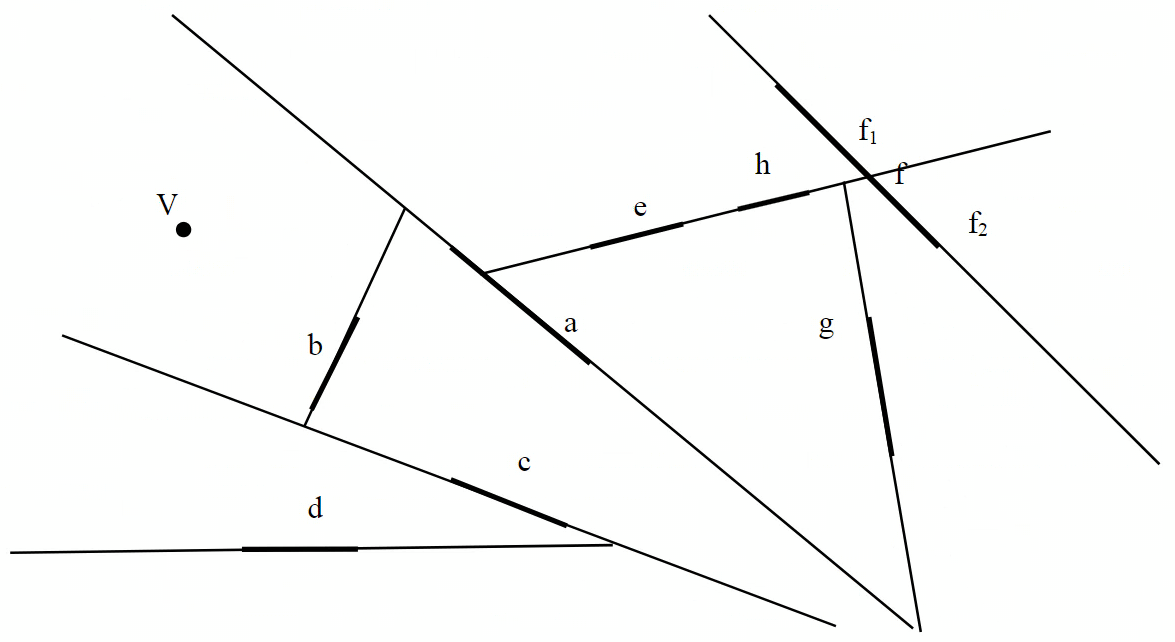
\includegraphics[width=0.9\textwidth]{artist3.png}		
	
		
	\end{frame}
	
	\section{Алгоритм трассировки лучей}
	
	\begin{frame}{Алгоритм трассировки лучей}
		\centering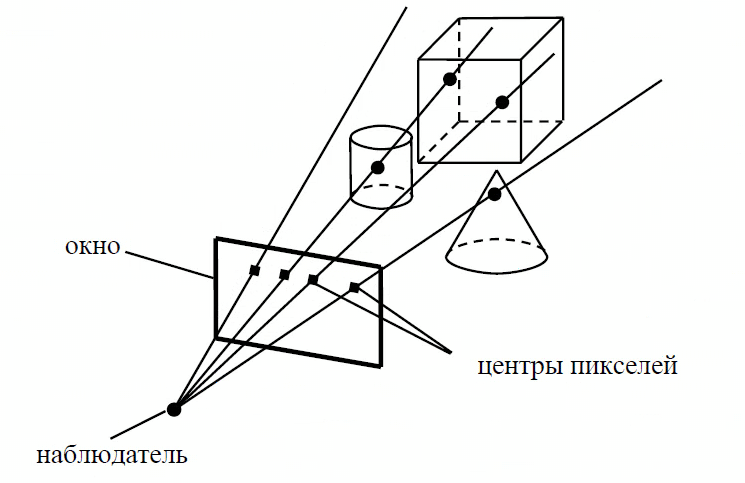
\includegraphics[width=0.9\textwidth]{raytrace.png}		
		
		
	\end{frame}
	
	\section{Алгоритм построчного сканирования}
	
	\begin{frame}{Алгоритм построчного сканирования}
		\centering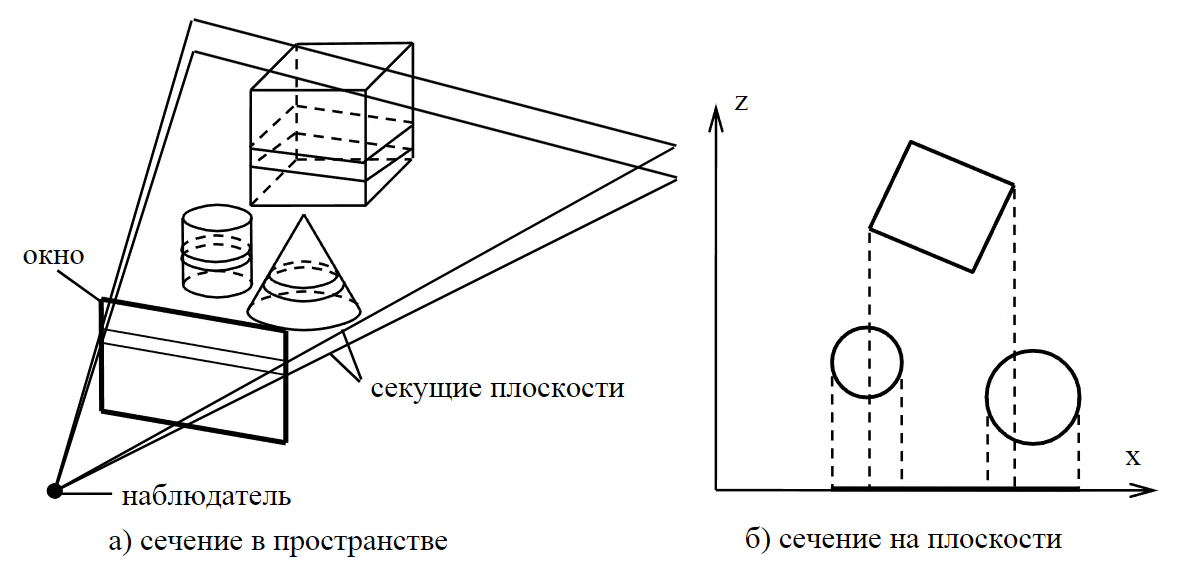
\includegraphics[width=0.9\textwidth]{string.png}			
		
	\end{frame}
	
	\section{Алгоритм S-буфера}
	
	\begin{frame}{Алгоритм S-буфера}
		\centering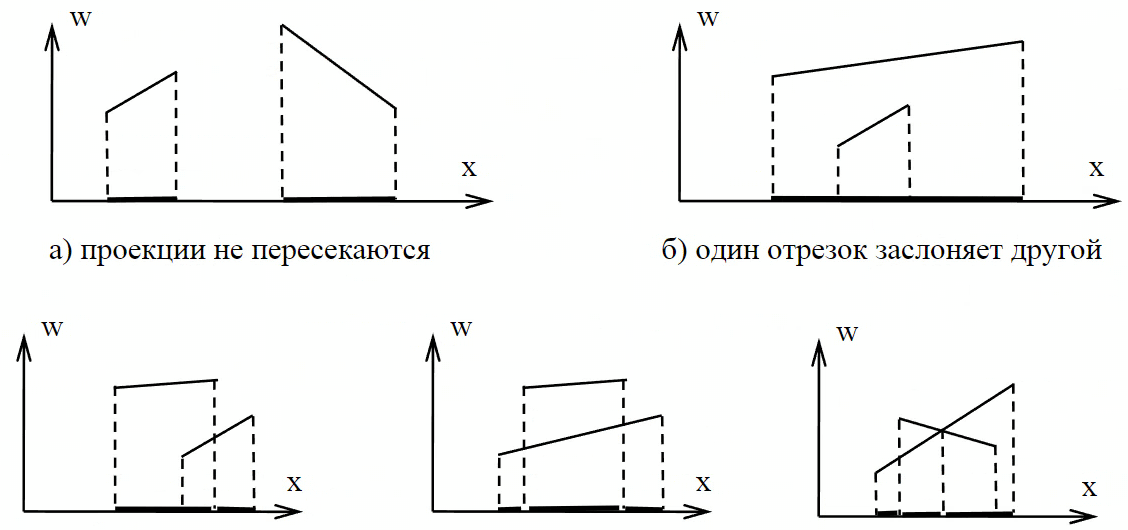
\includegraphics[width=0.9\textwidth]{sbuffer1.png}		
	\end{frame}
	
	\begin{frame}{Разбиение отрезков}
		\centering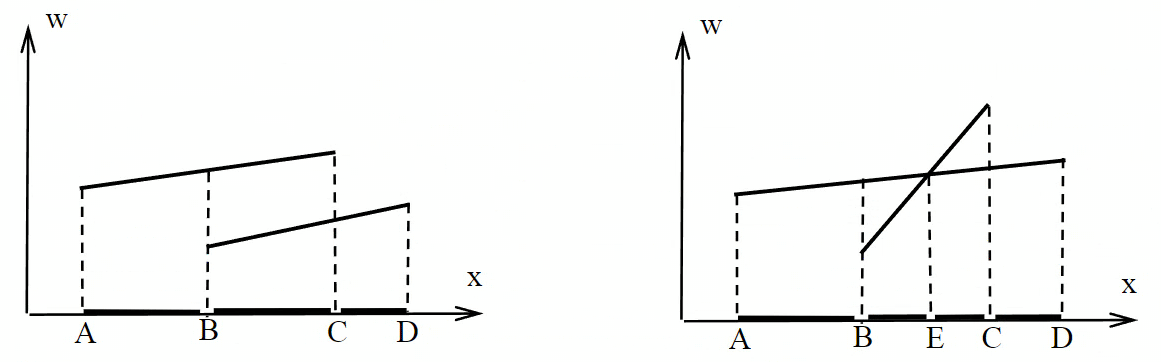
\includegraphics[width=0.9\textwidth]{sbuffer2.png}		
	\end{frame}
	
	
	

	
 
 
\begin{comment}
	
\end{comment}
 

\end{document}